\documentclass[tikz]{standalone}
\usepackage{pgfplots}
\usepackage{pgffor}
\usepackage{tikz-3dplot}
\usepgfplotslibrary{fillbetween}
\usepgfplotslibrary{patchplots}
\usetikzlibrary{3d}
\usepgfplotslibrary{colorbrewer} 
\tikzset{
  jumpdot/.style={mark=*,solid},
  excl/.append style={jumpdot,fill=white},
  incl/.append style={jumpdot,fill=black},
}
\usetikzlibrary{arrows.meta,intersections,calc,quotes,angles}
\pgfplotsset{width=7cm,compat=1.18} 
\begin{document}
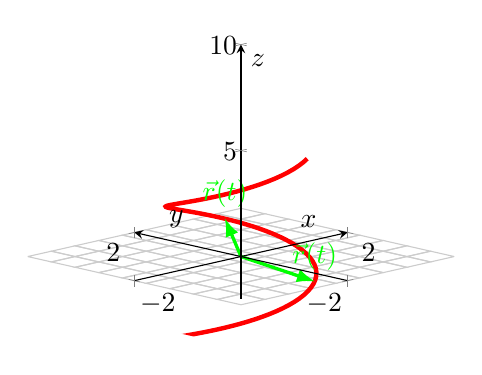
\begin{tikzpicture}
\begin{axis}[
  %comment below line to get "box" style 3d graph
  axis lines=center, 
  grid=major,
  axis on top,
  xmin=-2,
  xmax=2,
  ymin=-2,
  ymax=2,
  zmin=-2,
  zmax=10,
  xlabel=$x$,
  ylabel=$y$,
  zlabel=$z$,
  view={-45}{15},
  %%xtick={-3,0,...,5},
  %%ytick={-5,0,...,5},
  %%ztick={0,3,...,15},
  %xticklabel = \empty,
  %yticklabel = \empty,
  %zticklabel = \empty,
]

%xy grid lines
\addplot3[mesh, gray!40, samples=10, samples y=10, domain=-2:2, forget plot] {0};
\addplot3[no markers,red, samples=100, samples y=0, ultra thick] ({cos(x*57.2958)},{sin(x*57.2958)},{x});
\draw[green,-latex,very thick] (0,0,0) -- ({cos(57.2958)},{sin(57.2958)},1) node[above] {$\vec{r}(t)$};
\draw[green,-latex,very thick] (0,0,0) -- ({cos(-57.2958)},{sin(-57.2958)},-1) node[above] {$\vec{r}(t)$};

\end{axis}
\end{tikzpicture}
\end{document}